%!TEX program = xelatex
\documentclass{article}  

\usepackage[UTF8]{ctex}  
 
\usepackage[margin=1in]{geometry} 
\usepackage{amsmath,amsthm,amssymb}
\usepackage{parskip}
\usepackage{graphicx}
\usepackage{algorithm}
\usepackage[noend]{algpseudocode}
\usepackage{verbatim}
\usepackage{enumerate}
 
\newcommand{\N}{\mathbb{N}}
\newcommand{\Z}{\mathbb{Z}}


%%%%For macos users, please enable below commands to support chinese characters. If the fonts are not installed in your system, please install them first.
\setCJKmainfont{Kaiti TC Regular}
\setCJKsansfont{Songti TC Regular}
\setCJKmonofont{Heiti TC Regular}
 
\newenvironment{theorem}[2][Theorem]{\begin{trivlist}
\item[\hskip \labelsep {\bfseries #1}\hskip \labelsep {\bfseries #2.}]}{\end{trivlist}}
\newenvironment{lemma}[2][Lemma]{\begin{trivlist}
\item[\hskip \labelsep {\bfseries #1}\hskip \labelsep {\bfseries #2.}]}{\end{trivlist}}
\newenvironment{exercise}[2][Exercise]{\begin{trivlist}
\item[\hskip \labelsep {\bfseries #1}\hskip \labelsep {\bfseries #2.}]}{\end{trivlist}}
\newenvironment{reflection}[2][Reflection]{\begin{trivlist}
\item[\hskip \labelsep {\bfseries #1}\hskip \labelsep {\bfseries #2.}]}{\end{trivlist}}
\newenvironment{proposition}[2][Proposition]{\begin{trivlist}
\item[\hskip \labelsep {\bfseries #1}\hskip \labelsep {\bfseries #2.}]}{\end{trivlist}}
\newenvironment{corollary}[2][Corollary]{\begin{trivlist}
\item[\hskip \labelsep {\bfseries #1}\hskip \labelsep {\bfseries #2.}]}{\end{trivlist}}
 
\begin{document}
 
% --------------------------------------------------------------
%                         Start here
% --------------------------------------------------------------
 
%\renewcommand{\qedsymbol}{\filledbox}
 
\title{第二次作业}
\author{李亦杨 10195101467}
 
\maketitle

\section{}
\subsection{a}
见算法1.
\begin{algorithm}
\caption{rand$0.5$}
\begin{algorithmic}[1]
\Procedure{rand$0.5$}{}\Comment{以0.5概率输出true, 0.5概率输出false}
\While{true}
\State i = randP()
\State j = randP()

\If{i == 0 \&\& j == 1}
\State return true
\ElsIf{i == 1 \&\& j == 0}
\State return false
\EndIf
\EndWhile
\EndProcedure
\end{algorithmic}
\end{algorithm}

\subsection{b}

对于程序而言, 其仅有一个$while$循环. 在循环体内部, 首先对$randP$进行了两次调用, 随后进行$if$判断与继续循环. 由于给定的$ranP$以$p$概率输出$true$, 以$1-p$概率输出$false$, 因而$i == 0$且$j == 1$的情况概率为$p \cdot (1-p)$, 同时$i == 1$且$j == 0$的情况概率也为$p \cdot (1-p)$, 换言之每一次循环中, 能成功输出结果并跳出循环的概率为$2 \cdot p \cdot (1-p)$, 因而能成功输出结果的期望次数为$\frac{1}{2 \cdot p \cdot (1-p)}$, 由此可以计算得到, 该程序对$randP$的期望调用次数为:
\begin{align*}
expected\ &=\ 2 \cdot \ \frac{1}{2 \cdot p \cdot (1-p)} \\
&=\ \frac{1}{p(1-p)}
\end{align*}

\subsection{c}
如上所述, 程序的$while$循环内输出$true$的概率为$p \cdot (1-p)$, 输出$false$的概率也为$p \cdot (1-p)$, 因而可以保证程序以以$\frac{1}{2}$概率输出$true$, $\frac{1}{2}$概率输出$false$


\section{}
\subsection{a}
见算法2. 

\begin{algorithm}
\caption{FindMedian}
\begin{algorithmic}[1]
\Procedure{FindMedian}{A, B}
\State n $\gets$ the length of A
\State left = 0, right = n
\State median1 = 0, median2 = 0
\While{left $\leq$ right}
\State i = (left + right) / 2
\State j = (2n + 1) / 2 

\If{i == 0}
\State nums$\_$iml = INT$\_$MIN
\Else
\State nums$\_$iml = A[i - 1]
\EndIf
\If{i == n}
\State nums$\_$i = INT$\_$MAX
\Else
\State nums$\_$i = A[i]
\EndIf
\If{j == 0}
\State nums$\_$jml = INT$\_$MIN
\Else
\State nums$\_$jml = B[j - 1]
\EndIf
\If{j == n}
\State nums$\_$j = INT$\_$MAX
\Else
\State nums$\_$j = B[j]
\EndIf

\If{nums$\_$iml $\leq$ nums$\_$j}
\State median1 $\gets$ max(nums$\_$iml, num$\_$jml)
\State median2 $\gets$ min(nums$\_$i, nums$\_$j)
\State left = i + 1
\Else
\State right = i - 1
\EndIf
\EndWhile
\State return median1
\EndProcedure

\end{algorithmic}
\end{algorithm}
程序输入两个有序的长度为n的数组, 在$[0,n]$范围内进行二分查找, 找到满足一个特定条件$A[i-1] \leq B[j]$的$i$值, 从而得到对合并后数组进行中位划分的一种方法, 由此可以得到中位数

\subsection{b}
很显然, 中位数可以将一个数的集合划分为两个部分, 其长度相同(或前者比后者多一个), 同时前一部分中的元素总是小于等于后一部分中的元素 \\
换言之, 中位数划分的条件是:
\begin{align*}
len(left\_part) &= len(right\_part)\ +\ 1 \\
max(left\_part)\ &\leq \ min(right\_part) 
\end{align*}
为了确保这两个条件, 需要保证:
\begin{itemize}
\item $i\ +\ j\ =2n\ -\ i\ -\ j$($n$为偶数)或$i\ +\ j\ =2n\ -\ i\ -\ j\ +\ 1$($n$为偶数) \\
其中等号左侧为前一部分的元素个数,等号右侧为后一部分的元素个数. 由此可以计算得出$i\ +\ j\ =\ \frac{2n+1}{2}$
\item $0\ \leq \ i\ \leq \ n,0\ \leq \ j\ \leq \ n, $这样对于任意的$i\ \in \ [0,n]$, 都有$j\ =\ \frac{2n+1}{2}\ -\ i\ \in \ [0,n]$, 因而只要在$[0,n]$范围内枚举$i$得到$j$
\end{itemize}
假设$A[i-1], B[j-1],A[i],B[j]$永远存在, 临界条件时取正无穷与负无穷以防止对最值判断产生影响即可. 因而只要在$[0,n]$中找到$i$使:
\begin{align*}
B[j-1]\ \leq \ A[i]\ and\ A[i-1]\ \leq \ B[j], \\
j\ =\ \frac{2n+1}{2}\ -\ i
\end{align*}
这是因为这与在$[0,n]$中找到最大的$i$使:
\begin{align*}
A[i-1]\ \leq \ B[j], \\
j\ =\ \frac{2n+1}{2}\ -\ i
\end{align*}
等价. 因:
\begin{itemize}
\item 当$i$从$0\ \sim \ n$递增时, $A[i-1]$递增, $B[j]$递减, 因而存在最大的$i$满足$A[i-1]\ \leq \ B[j]$
\item 如果$i$是最大的, 那么$i+1$不满足, 因而$B[j-1]\ \leq \ A[i]$成立, 与变换前相同
\end{itemize}
因而只需在$[0,n]$范围内进行二分查找, 找到满足一个特定条件$A[i-1] \leq B[j]$的$i$值, 从而得到对合并后数组进行中位划分的一种方法, 由此可以得到中位数.

\subsection{c}
根据程序可以得知, 进行二分查找的区间为$[0,n]$, 该区间每次循环长度变为原来的一半, 因而只需要执行$log(n)$次循环. 因而时间复杂度为$O(log(n))$. 


\section{Sorting in Linear Time}
\subsection{a}
见算法3. 

\begin{algorithm}
\caption{SortPair}
\begin{algorithmic}[1]
\Procedure{SortPair}{A}\Comment{A是数对序列}
\State match A to Ab, where Ab is a sequence of the second entries in A \Comment{将A与Ab作一一映射, Ab代表数对序列A中后一项$b_n$形成的数列}
\State match A to Aa, where Aa is a sequence of the first entries in A \Comment{将A与Aa作一一映射, Aa代表数对序列A中前一项$a_n$形成的数列, 此句和上句可以通过构造一个结构体实现}
\State CountSort(Ab)\Comment{对Ab进行计数排序, 通过映射可以保证A同时被按数对后一项排序}
\State CountSort(Aa)\Comment{对Aa进行计数排序, 通过映射可以保证A同时被按数对前一项排序}
\State return A
\State
\EndProcedure

\Procedure{CountSort}{A}\Comment{A是一个数列, 结果升序排列}
\State max $\gets$ the maximum entry in A
\State min $\gets$ the minimum entry in A
\State len = max - min + 1
\State initialize array couarr of length len
\For{i in A}
\State couarr[arr[i] - min] ++ \Comment{统计元素个数}
\State sum = 0
\EndFor
\For{i in couarr}
\State sum += couarr[i]
\State couarr[i] = sum
\EndFor
\For{i in A, from the last to the first}\Comment{倒序遍历原数组}
\State sortarr[couarr[arr[i] - min] - 1] = arr[i]
\State couarr[arr[i] - min] -- \Comment{下次遇到相同值的内容往前排一位}
\EndFor
\EndProcedure
\end{algorithmic}
\end{algorithm}
正确性证明: \\
首先考虑计数排序的正确性证明. \\
\begin{enumerate}[1)]
\item 显然对于任何大小为空或$1$的数组, 计数排序算法总能给出正确的排序结果, 且总能保证其是稳定的 
\item 现在假设排序在不超过k个元素的所有数组上都是稳定的排序 \\
考虑一个大小为$k+1$的数组, 这个数组有一个最大的最后一个元素(在排序标准最大的元素中,有一个出现在数组的最后). 考虑通过从大小为$k+1$的数组中删除此元素并将出现在其右侧的元素向左移动以填补空白而获得的大小为$k$的数组. 根据归纳假设, 计数排序在这个大小为$k$的数组上是稳定的. \\
为了证明计数排序在大小为$k+1$元素的数组上是稳定的, 因此必须证明计数排序不能将最大的最后一个元素放在任何相同大小的元素之前. 不难看出这是因为,在构造输出数组 $B$时,$j$假定值$n, n-1, ..., 1$按降序排列,因此在所有与最大的最后一个元素具有相同值的元素中, 它将首先到达我们的元素. 因此, 可以保证将此元素放置在$B$中比放置具有相同值的任何其他元素更靠右的位置, 因为 $C[A[j]]$在构造 B 的循环中递减. 
\item 由此可以证明计数排序是一个稳定的排序算法
\end{enumerate}
现在来考虑算法$SortPair$, 其对数列进行两次对计数排序的调用, 先对数对后者进行计数排序, 再对数对前者进行计数排序. 前面已经证明了计数排序是一个稳定的排序算法, 由于先对数对后一项进行计数排序, 在对前一项进行第二次排序时, 计数排序的稳定性保证了对数对序列中拥有值相同的前一项的数对, 其后一项保持着第一次排序的相对顺序(即位置不交换), 因而在进行两次排序后可以保证输出一个能够满足以 lexicographic order 排序的数对序列. \\
现在来考虑其时间复杂度: \\
同样, 首先先计算计数排序的时间复杂度. 对计数排序而言, 其一共你醒了三次$for$循环, 第一次$for$循环遍历输入的数组, 其大小为$n$, 第二次遍历大小为$len\ =\ max\ -\ min\ +\ 1$的数组, 第三次再次遍历输入数组, 因而其时间复杂度为: 
\begin{align*}
T(n)\ &=\ O(n)\ +\ O(l)\ +\ O(n) \\
&=\ O(n\ +\ k)
\end{align*}
而算法$SortPair$对计数排序进行了两次调用, 因而可以计算其时间复杂度为:
\begin{align*}
O(n\ +\ k)\ +\ O(n\ +\ k)\ =\ O(n)
\end{align*}

\subsection{b}
对于范围$[0,n^2)$内的全部数$k$, 考虑其不为质数的情况, 那么其可以被拆分为两个数$a_k, b_k$, 我们对其进行排序保证前一个数永远小于后一个数, 并保证两个数尽量接近, 显然我们可以发现$a_k\leq n$, 且后一个数组成的数列其最大最小值之差不会超过2n, 而对于质数, 可以将其拆分为$1 \cdot k$的形式, 并将第一项为$1$的全部数单独进行计数排序, 而不参与到数对排序的第一次排序中, 并在数对排序的第二次排序后将其置于最前, 我们也显然可以知道质数的数量不会超过n, 因而可以保证这样的排序时间复杂度为$O(n)$.


\section{}
\subsection{(a)}
\subsubsection{(i)}
第一个树可以作为红黑树结构, 如下图 \\
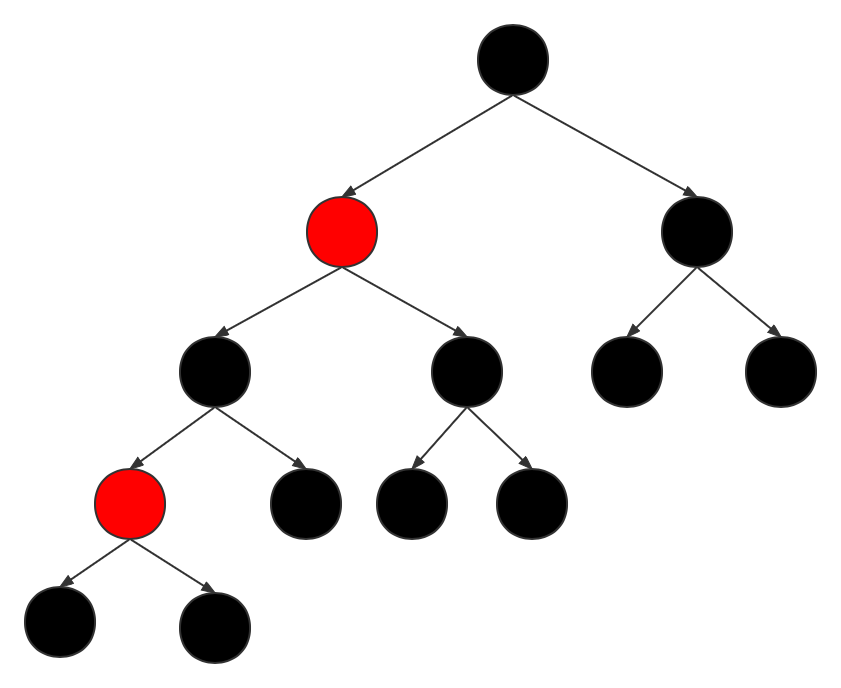
\includegraphics[scale=0.4]{Figure1.png}
\subsubsection{(ii)}
第二个树不能满足第四条性质, 即不能满足每条路径上有相同数量黑色结点. \\
这是因为, 考虑到根结点右子树最长路径含三个结点(含根结点), 左子树最长路径含五个结点, 因而根结点的左孩子(记为结点a)必须被染成红色(此时从根结点到叶子结点必须含3个黑色结点), 也因此a的右孩子b必须为黑色. 为了保证从根结点到b左孩子这条路径含3个黑色结点, b的左孩子必须为黑色, 然而此时从根结点到b的黑色结点数为2, 不符合第四条性质, 因而这一个树不能作为红黑树结构

\subsection{(b)}
\subsubsection{(i)}
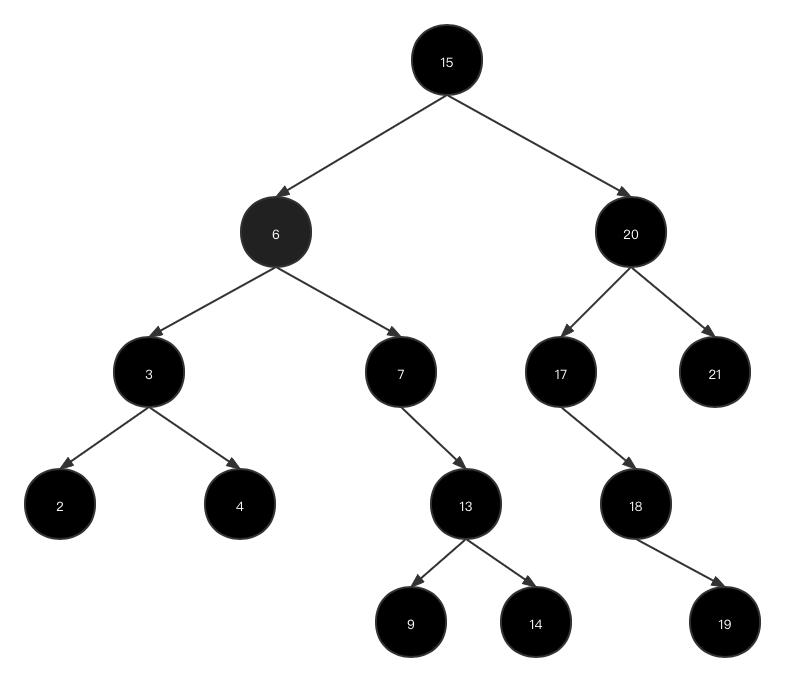
\includegraphics[scale=0.4]{Figure2.png}
\subsubsection{(ii)}
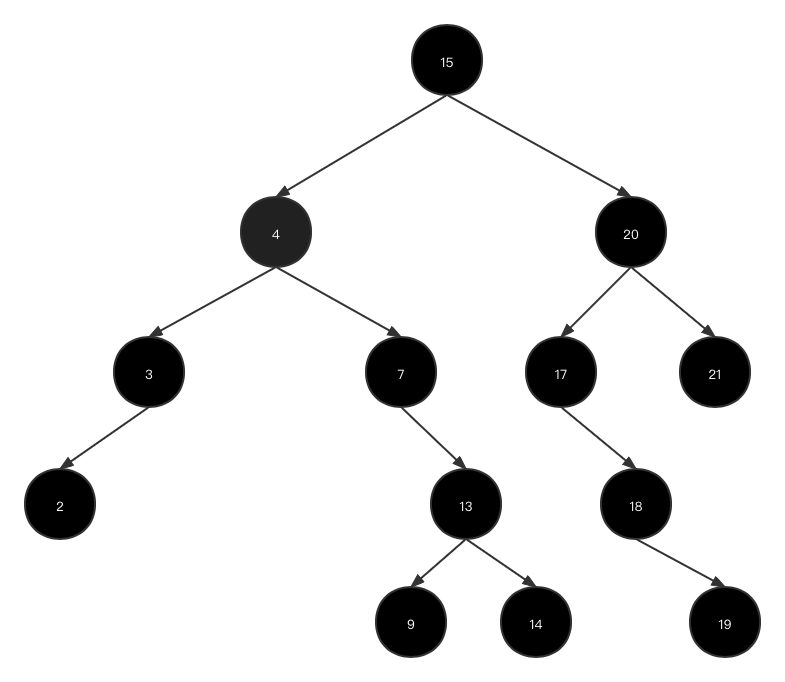
\includegraphics[scale=0.4]{Figure3.png}
\subsubsection{(iii)}
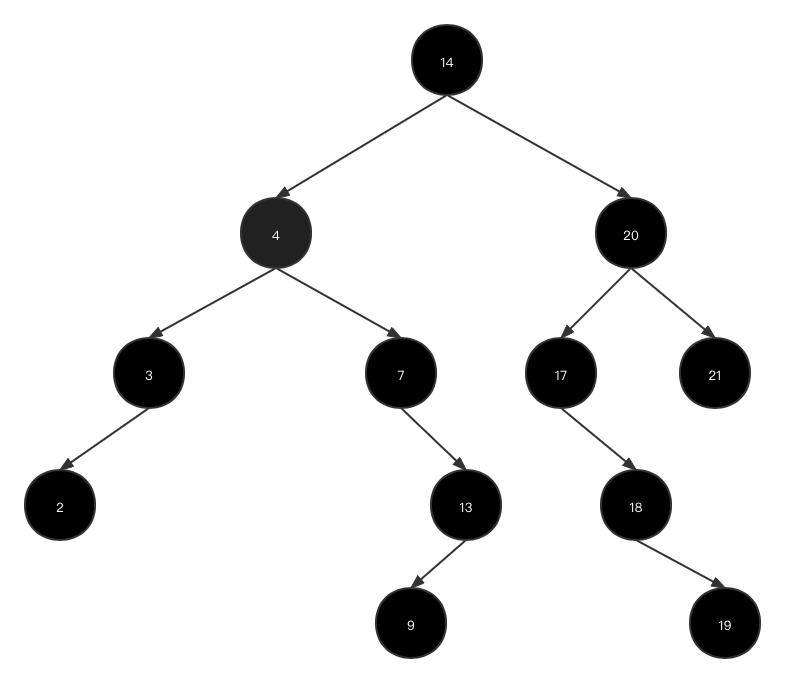
\includegraphics[scale=0.4]{Figure4.png}


\section{}
\subsection{(a)}
这一断言显然是错误的. 下图即是一个反例: \\
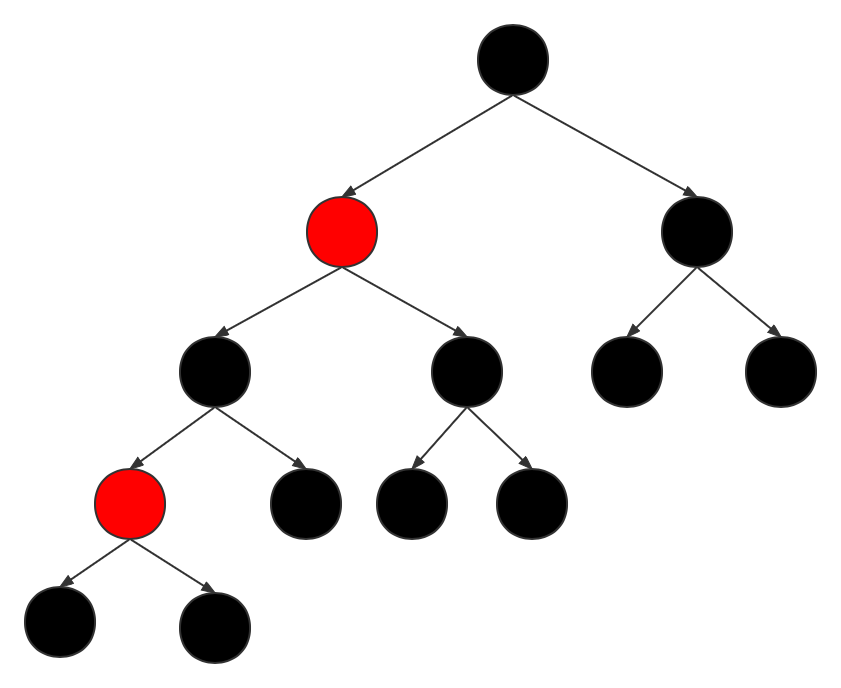
\includegraphics[scale=0.25]{Figure1.png} \\
该反例中, 总结点为12, 按照断言理应左右子树结点数都大于等于5, 然而右子树仅有三个结点

\subsection{(b)}
考虑较为极端的情况, 换言之假设右子树全为黑色结点, 高度为$x$(不包括根结点), 其含有结点数为$2^x-1$, 那么此时左子树高度为$2(x+1)-1-1 = 2x$, 最多含有结点数为$2^{2x}-1$, 因而此时有:
\begin{align*}
2^{2x}\ -\ 1\ +\ 1\ +\ 2^x\ -\ 1\ &=\ |T| \\
(2^{x})^2\ +\ 2^x\ +\ 1\ &=\ |T| \\
(2^x\ +\ \frac{1}{2})^2\ &=\ |T|\ -\ \frac{3}{4} \\
2^x\ &=\ \frac{\sqrt{4|T|-3}}{2}\ -\ \frac{1}{2} \\
&\geq \ \frac{\sqrt{|T|}}{2}\ -\ 1
\end{align*}
换言之此时有:
\begin{align*}
|T_R|\ \geq \ \frac{\sqrt{|T|}}{2}\ -\ 1
\end{align*}
由对称性可知, 
\begin{align*}
|T_L|\ \geq \ \frac{\sqrt{|T|}}{2}\ -\ 1
\end{align*}


\section{}
根据假设, 可以假设所有的键都是完全有序的$\{k_1, k_2, ..., k_m\}$, 由于哈希是简单且均匀的, 因而每进行一次插值其不发生碰撞的可能性为$\frac{i-1}{m}$, 其中$i$为代表进行第$i$次插入, 换言之其不发生碰撞的概率为$\frac{m-i+1}{m}$, 从而可以得出期望的不发生碰撞的次数为:
\begin{align*}
\sum_{i=1}^n1 \cdot\ \frac{m-i+1}{m}\ &=\ 1\ +\ \frac{m-1}{m}\ +\ \frac{m-2}{m}\ +\ ...\ +\ \frac{m-n+1}{m} \\
&=\ n\ -\ \frac{n^2-n}{2m} \\
&=\ \frac{2nm-n^2+n}{2m}
\end{align*}
而最大的不碰撞次数显然发生在每一次插入均不发生碰撞的情况, 换言之对$n$次插入最大的不碰撞次数为$n$


\end{document}